\section{System Design}
\label{sec:system_design}
\subsection{Embedded system architecture}
The system architecture is an embedded CPU+FPGA-based platform illustrated in \fig{fig:system_architecture}. The CPU communicates with the tensor accelerator (TA) trough AXI-Lite, and the TA communicates to the external memory though AXI-Stream interface via Direct Memory Access (DMA).
\begin{figure}[t!]
	\centering
	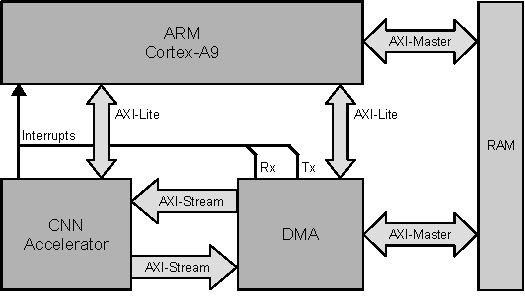
\includegraphics[width=0.5\textwidth]{../figures/system_design.pdf}
	\caption{System-level architecture of the proposed embedded platform.}
	\label{fig:system_architecture}
\end{figure}

\subsection{Tensor accelerator}
The tensor accelerator is a dedicated hardware module to compute tensor operations. In this paper, we present Conv2D and DepthwiseConv2D operators implemented using HLS with an approximate computing approach. For each operator, the compute engine represents the TFLite micro kernel C++ code adapted for hardware HLS. The accelerator architecture is illustrated in \Fig{fig:accelerator}.

\begin{figure}[t!]
	\centering
	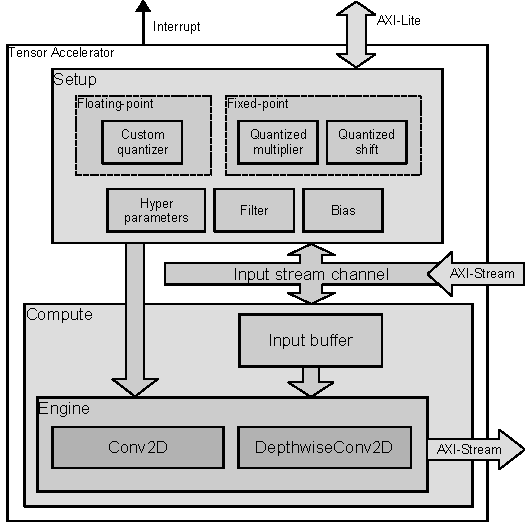
\includegraphics[width=0.5\textwidth]{../figures/accelerator.pdf}
	\caption{Hardware architecture of the proposed accelerator.}
	\label{fig:accelerator}
\end{figure}

This accelerator offers two modes of operation: \emph{configuration} and \emph{computation}.

\subsubsection{Setup mode}
In this mode, the accelerator receives the tensor operator ID and the hyperparameters for execution: stride, dilation, padding, offset, activation, quantized activation, depth-multiplier, input shape, filter shape, bias shape, and output shape. Afterwards the accelerator receives: filter tensor, bias tensor, and quantized multiplier/shift vectors in the case of using 8-bit quantization. These hyperparameters and tensors are stored in on-chip memory for reusage during compute mode.

\subsubsection{Computation mode}
In this mode, the accelerator performs the tensor operator according to the hyperparameters received during setup mode.

\subsection{Compatibility}

 This hardware accelerator is compatible with TF Lite 8-bit quantized and floating-point formats. The designer is able to select the compute and number formats prior hardware synthesis.
 
 \subsection{Dot-product computation}
Internally, the accelerator performs floating-point computation employing either: (1) HLS Xilinx LogiCORE IP, (2) decomposed custom floating-point, and (3) logarithmic computation. This design is proposed in \cite{nevarez2021accelerating}, where the authors present the hybrid custom floating-point and logarithmic dot-product approximation to accelerate Spike-by-Spike neural networks on embedded FPGA. In this paper, we adopt this approach to accelerate the vector dot-product on the convolution operators. With this approach, the designer is able to select the desired vector dot-product. See \Fig{fig:dot_product}.

\begin{figure}[t!]
	\centering
	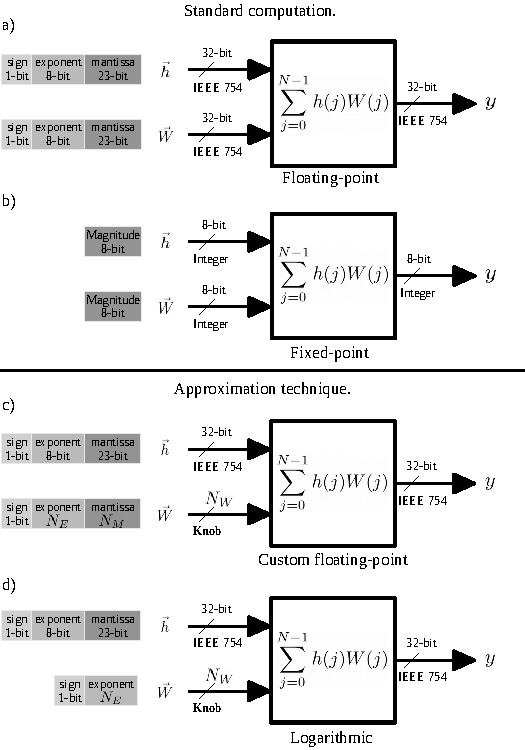
\includegraphics[width=0.5\textwidth]{../figures/dot-product_unit.pdf}
	\caption{Hardware alternatives for vector dot-product.}
	\label{fig:dot_product}
\end{figure}


\subsection{Embedded software architecture}
The software architecture is an extended version of TFLite for microcontrollers\cite{TensorFlowLibrary}. We implemented a delegate class for TFLite. This class encapsulates the accelerator and DMA low-level drivers. The TFLite library delegates the  Conv2D and DepthwiseConv2D tensor operations to the hardware accelerator, while the rest of the tensor operators are executed on the embedded CPU. At the application level, the end user would use the regular TFLite application programming interface (API) to load TFLite models, set input tensors, invoke inference, and get output tensors. The overall structure is depicted in \fig{fig:sw_stack}.

\begin{figure}[t!]
	\centering
	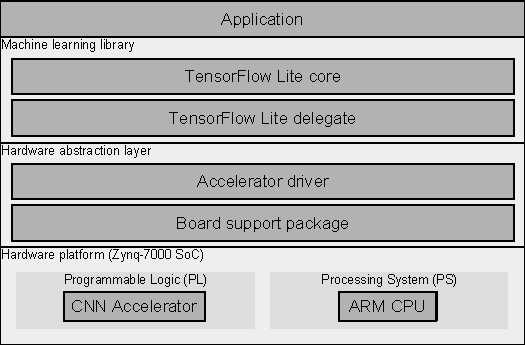
\includegraphics[width=0.5\textwidth]{../figures/sw_stack.pdf}
	\caption{System-level overview of the embedded software architecture.}
	\label{fig:sw_stack}
\end{figure}
